\documentclass[12pt]{article}

% Language setting
% Replace `english' with e.g. `spanish' to change the document language
\usepackage[english]{babel}

% Set page size and margins
% Replace `letterpaper' with `a4paper' for UK/EU standard size
\usepackage[letterpaper,top=1cm,bottom=1.25cm,left=1cm,right=1cm,marginparwidth=1.75cm]{geometry}

% Useful packages
\usepackage{amsmath}
\usepackage{amssymb}
\usepackage{graphicx}
\usepackage{caption}
\usepackage{subcaption}
\usepackage[colorlinks=true, allcolors=blue]{hyperref}
\usepackage{indentfirst}
%\usepackage{biblatex}
\usepackage{titling}

%Importing the library needed to support code displaying
\usepackage{listings}
\usepackage{color}
\captionsetup{font=small}

\title{Patch Antenna Design and Miniaturization Techniques \\A Qualitative Approach}
\author{Andrey Lototskiy}
\date{\today}

\begin{document}
\maketitle

\begin{abstract}
Hello world!
\end{abstract}

\section{Introduction}
Among all of the antennas in use today, perhaps none is as revolutionary as the patch antenna. First envisioned in the 1950's\cite{gutton1955flat}, patch antennas were first adopted by the aerospace industry\cite{balanis2016antenna}, due to their low profile and light weight being essential for spacecraft, missiles, and airplanes. In the 1980's, with the advance of printed circuit technology, patch antennas became far cheaper to manufacture\cite{khan2015microstrip}, which brought them applications in commercial wireless communication systems. 
However, these very rudimentary patch antennas were too large to be effectively used in hand held devices. Like all antennas, patch antennas (PAs) radiate most efficiently when their length is one-half of the wavelength they emit \cite{khan2015microstrip}. For instance, if one wanted to design a PA which radiated at a frequency of $900$ MHz, then, without using any of the miniaturization techniques discussed in this paper, they would need their PA to have a length of around $33$ cm, which is too big to be used in many applications. 

\begin{figure}[h]
    %\begin{subfigure}{0.5\textwidth}
    \centering
    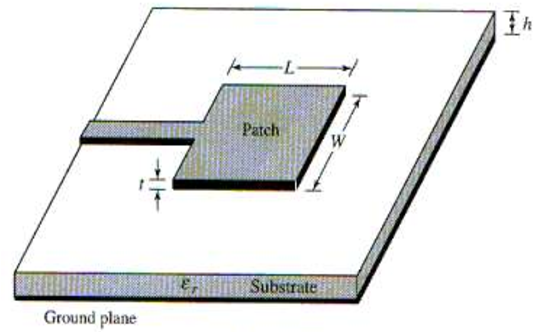
\includegraphics[width=0.5\textwidth]{patch-antenna-structure.png}
    %\end{subfigure}
    \caption{The basic structure of a patch antenna. This particular antenna is being fed with a microstrip. The ground, and the patch are conductors. The substrate is a dielectric. \cite{girase2014design}}
\end{figure}

Besides its large size at lower frequencies, a PA with Figure 1's design would have a narrow frequency band, low efficiency, low power, high Q, poor polarization purity, and spurious feed radiation\cite{balanis2016antenna}. Fortunately, significant effort has gone into addressing these limitations, and a variety of design techniques to mitigate these limitations have been created\cite{balanis2016antenna}. Furthermore, PAs have also been investigated theoretically, and theories to describe the operating mechanism of most PAs have been created. However, the theories describing PA operation are mathematically dense. Furthermore, some of them make     
  
\section{Patch Antenna}

\subsection{Basic Characteristics}

\newpage
\bibliographystyle{IEEEtran}
\bibliography{main}
%\printbibliography


\end{document}
